\documentclass[12pt]{article}
\usepackage{amsmath}
\usepackage{amssymb}
\usepackage{geometry}
\usepackage{enumerate}
\usepackage{natbib}
\usepackage{float}%稳定图片位置
\usepackage{graphicx}%画图
\usepackage[english]{babel}
\usepackage{a4wide}
\usepackage{indentfirst}%缩进
\usepackage{enumerate}%加序号
\usepackage{multirow}%合并行
\title{\large UM-SJTU JOINT INSTITUTE\\Electronic Circuits\\(VE311)\\\ \\\ \\\ \\\ \\\ \\\ \\\ \\\ \\\ \\\ \\\
LABORATORY REPORT\\\ \\\ LAB 2\\\  \\\ \\\ \\\ \\\ }
\author{Name: Pan Chongdan\\\ Name: Wang Xinyi \\\ Name: Shen Yinchu \\\ Name: Zhang Zhengyuan}
\date{Date: \today}

\begin{document}
 \maketitle
\newpage
\section{Common-Emitter Amplifier}
\begin{enumerate}[(a)]
\item First, we chose a resistor of 15 $\Omega$ and then we chose a resistor of $5000\Omega$, but the start voltage is always not $5V$ and it didn't change much as we performed the DC sweep. Then we found the ground voltage for $V_{CC}$ and $V_{in}$ is not same, so we used wires to put the ground together. Then as we increased the resistor until it's 90000$\Omega$, the $V_{out}$ at $V_{in}=0$ is at $5V$.
\begin{figure}[H]
\centering
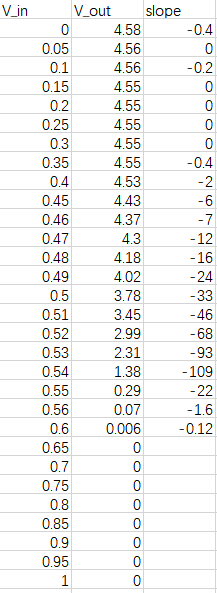
\includegraphics[scale=0.5]{P1.png}
\caption{experiment data}
\end{figure}
\par We first did the DC sweep with each interval equals $0.05V$, and then we found there is an brutal change when the $V_{\textrm{in}}$ is from $0.45V$ to $0.55V$, than we did the sweep with the interval equals $0.01V$ and calculated the slope. In the end, we chose $V_{\textrm{in}}$ as $0.47V$
\begin{figure}[H]
\centering
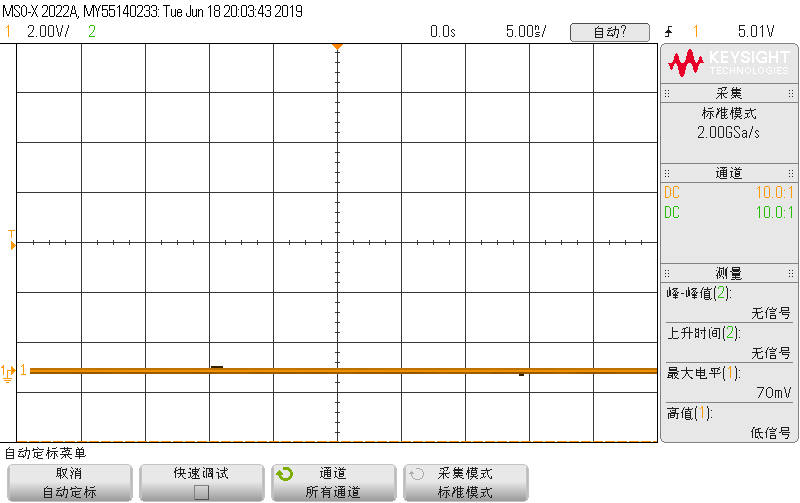
\includegraphics[scale=0.5]{P2.png}
\caption{experiment data}
\end{figure}
This is the figure as we did the DC sweep, but we found there is some error between the oscilloscope and potentiometer. The potentiometer is more accurate as we tried to get the DC value. We thought the reason behind this phenomenon is the internal resistor or oscilloscope is not designed to measure the DC value.
\item
\begin{figure}[H]
\centering
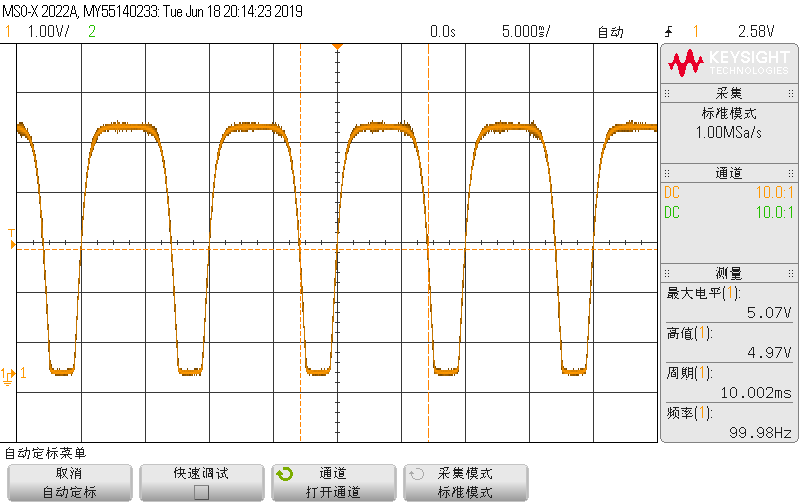
\includegraphics[scale=0.5]{P3.png}
\caption{(b) figure}
\end{figure}
This is the figure from oscilloscope when $V_{in}=V_{\textrm{in}}+0.1\sin(2\pi10^2\cdot \textrm{time})$ the amplitude of $v_{out}$ is close to $0.1A_v$. However, the figure is not symmetric horizontally, so we decided to change the $V_{\textrm{in}}$ amplitude and saw the figure. We observed that some parts will appear on the figure so the figure is symmetric. We thought it's because the $V_{\textrm{in}}$ is too big so that the total figure can't be shown on the oscilloscope completely.
\item
\begin{figure}[H]
\centering
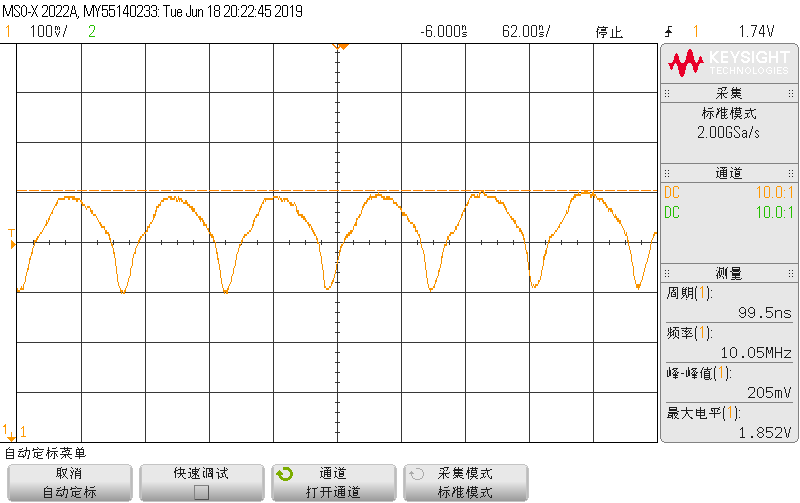
\includegraphics[scale=0.5]{P4.png}
\caption{(c) figure}
\end{figure}
This is the figure from oscilloscope when $V_{in}=V_{\textrm{in}}+0.1\sin(2\pi10^7\cdot \textrm{time})$ the amplitude of $v_{out}$ is much smaller than $0.1A_v$. We thought it's because $v_{out}$ can't reach the amplitude that it should reach in time because of the high frequency. Also, we found that the figures seems to drift on the screen so we decreased the frequency slowly and found the figures didn't appear to drift any more. So we think the frequency is too high for the BJT to react and from the Internet, we found some BJT do have a react frequency about 10MHz, which is our frequency and as a result, the $v_{out}$ can't reach its amplitude.
\end{enumerate}

\end{document}